\documentclass{article} % For LaTeX2e
% We will use NIPS submission format
\usepackage{nips13submit_e,times}
% for hyperlinks
\usepackage{hyperref}
\usepackage{url}
% For figures
\usepackage{graphicx} 
\usepackage{subfigure} 
% math packages
\usepackage{amsmath}
\usepackage{amsfonts}
\usepackage{amsopn}
\usepackage{ifthen}
\usepackage{natbib}

\title{Project-I by Group Sydney}

\author{
Diego Antognin and Jason Racine \\
EPFL \\
\texttt{diego.antognini@epfl.ch}, \texttt{jason.racine@epfl.ch} \\
}

% The \author macro works with any number of authors. There are two commands
% used to separate the names and addresses of multiple authors: \And and \AND.
%
% Using \And between authors leaves it to \LaTeX{} to determine where to break
% the lines. Using \AND forces a linebreak at that point. So, if \LaTeX{}
% puts 3 of 4 authors names on the first line, and the last on the second
% line, try using \AND instead of \And before the third author name.

\nipsfinalcopy 

\begin{document}

\maketitle

\begin{abstract}

\end{abstract}

\section{Regression}

\section{Data Description}

The train-data for regression consists of $N = 2800$ input ($\mathbf{X}$) and output ($\mathbf{y}$) data samples. Each input sample is a vector $\mathbf{x}_n$ with dimension $D = 76$. Out of these $76$ variables, $63$ are real, $3$ binary, $4$ categorical with 3 categories, $6$ are categorical with 4 categories.

We also have test-data of size $N=1200$ without their corresponding output. Our goal is to produce predictions for those data, as well as an approximation of the test-error.

\section{Data visualization and cleaning}

NORMALIZED ALL DATA OR NORMALIZATION PER CLUSTER ?

We first have plot the distribution of our features (plot not shown because too big for the $76$ features). As expected, they are not center and we should normalized them. The Figure \ref{fig:histogram} shows an histogram of the output ($\mathbf{y}$) and we can conclude our data  seem to be a combination of three Gaussian distributions. It will be used later in order to separate the data in three sets and apply different regression models on them. We can also observe that each cluster have different sizes : 1946, 576 and 278. Moreover, on the right, we can see some data points (there are $2$) which have a higher values than the others. We consider them as outliers and we will remove.

To separate the data, we have observed that the feature $2$ and $16$ could help us. Figure \ref{fig:feature2}. We can observe $11$ misclassified data (green points), which we will remove them in order to not corrupt our model.  So, this feature can allow us to find the first cluster. For the two others clusters, we need to oberve the feature $16$. Figure \ref{fig:feature16}. We can observe $14$ misclassified data (green points and one blue). They also will be consider as outliers and remove. We set the threshold in order to minimize the number of misclassified data samples. Those thresholds are $0.42$ for the feature $2$ and $1.17$ for the feature $16$.

We are also interested about the correlation between the input and output variables. We have observed the correlation for each cluster and conclude that for the first cluster, they are mainly in $[-0.1,0.1]$, except two features which are highly correlated. For the second and third cluster, also mainly in $[-0.1,0.1]$ but this time, there are more correlated features (~15). Moreover, the features seem not have correlation between them.

ENCODING CATEGORICAL FEATURES

We can note that the rank of our input matrix $\mathbf{X}$ is rank-deficient with a rank of 66 instead of 76.

\begin{figure}[!t]
\center
\subfigure[Histogram of $\mathbf{y}$. We can see three Gaussian distributions and also some outliers on the right.]{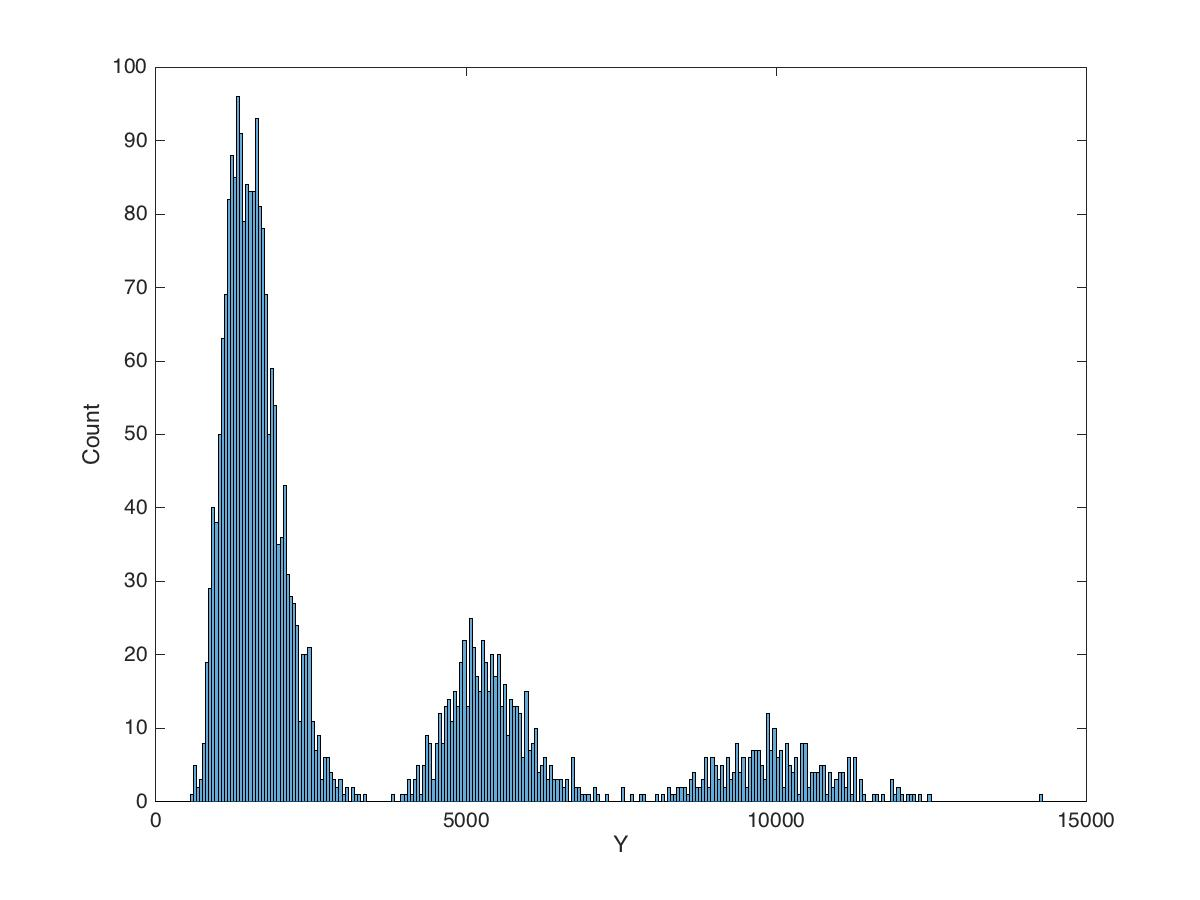
\includegraphics[width=2.5in]{figures/histogram.jpg} \label{fig:histogram}}
\hfill
\subfigure[Feature 2, because we have assumed that the data was generated from three Gaussian, this feature can help us to separate the data. Green data points are misclassified data. The separation is at $x=0.42$.]{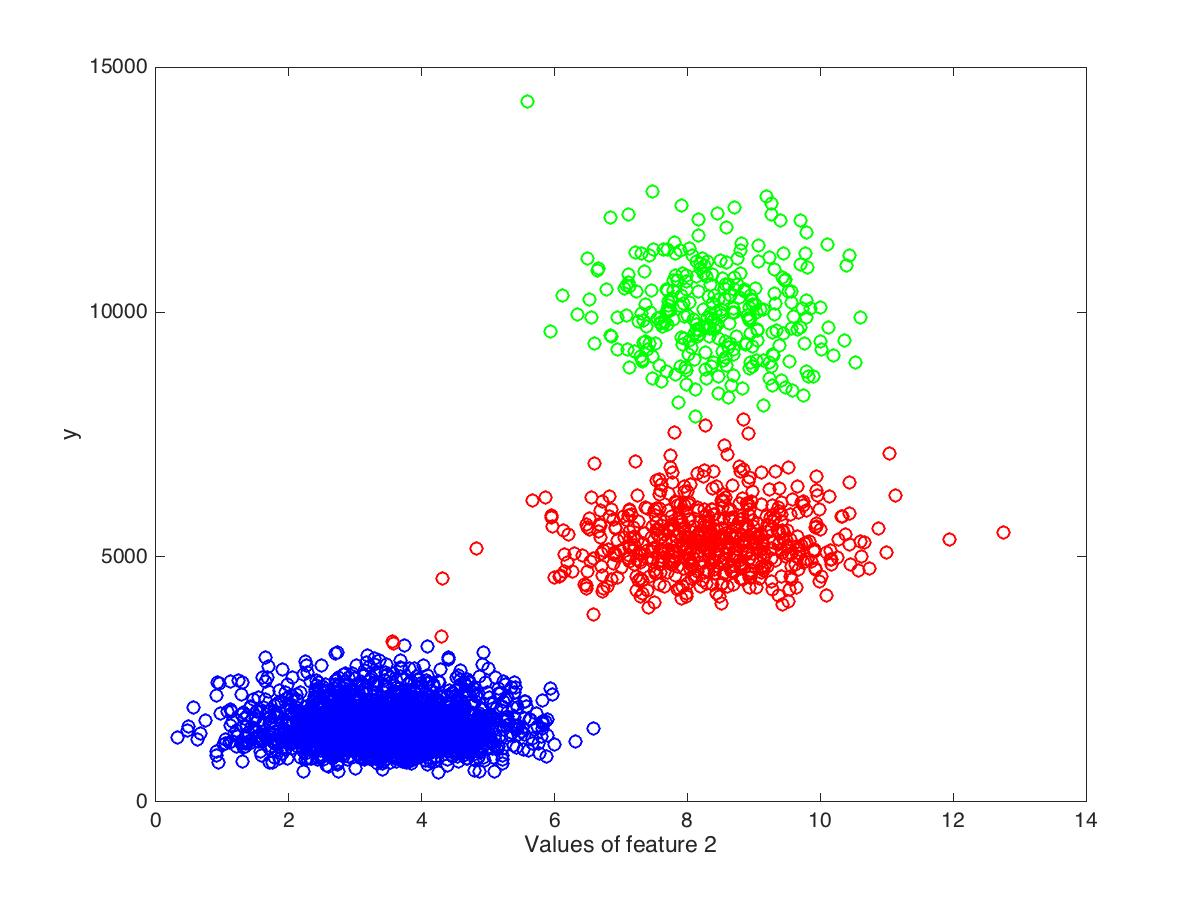
\includegraphics[width=2.5in]{figures/feature2.jpg}\label{fig:feature2}}
\hfill
\subfigure[Feature 16, because we have assumed that the data was generated from three Gaussian, this feature can help us to separate the data. Green data points are misclassified data. We can see see a blue data point which is misclassified, it will be an outlier. The separation is at $x=1.17$.]{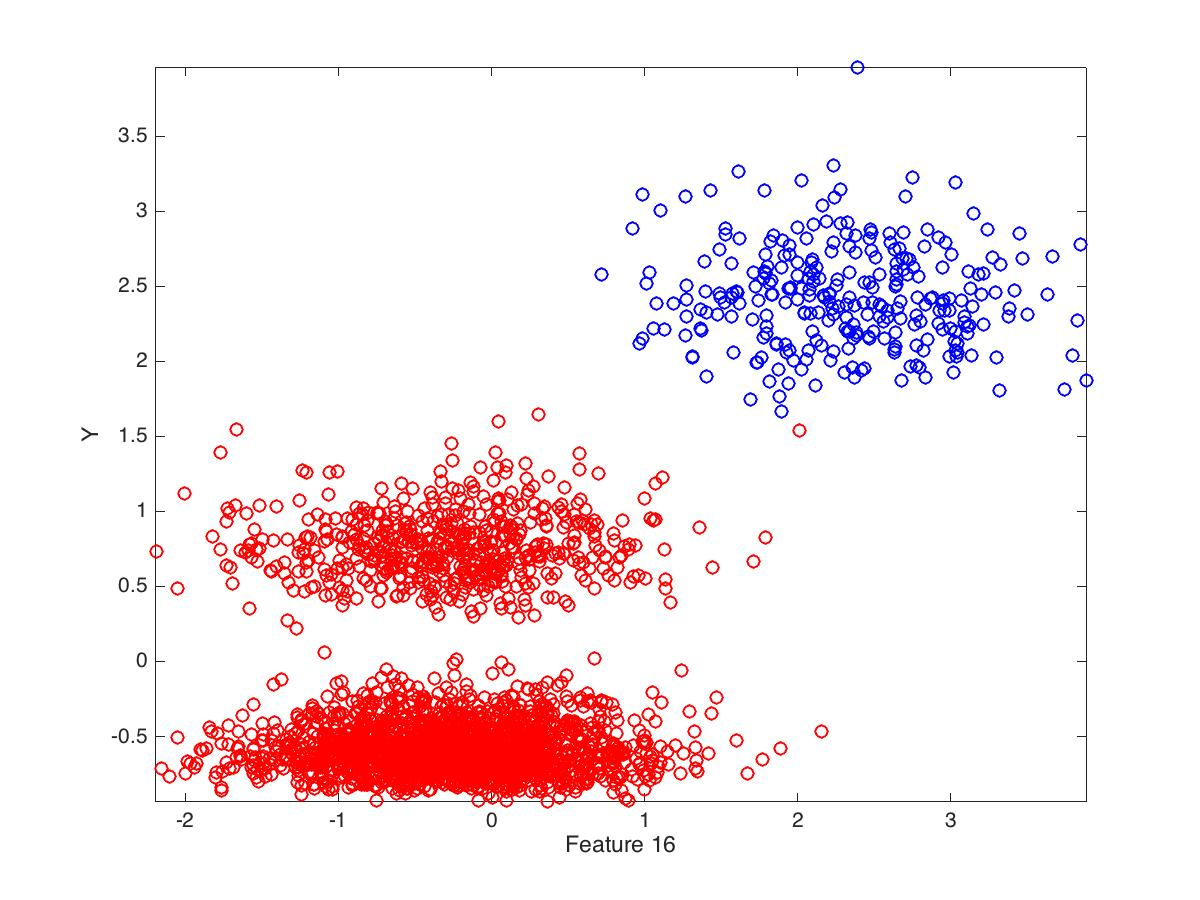
\includegraphics[width=2.5in]{figures/feature16.jpg}\label{fig:feature16}}
\hfill
\caption{}
\end{figure}

\end{document}
